\subsection{La \eng{rasterisation}\label{sec:rasterization}}
Encore aujourd'hui, la méthode privilégiée de visualisation 3D est la
\eng{rasterisation}. Cette technique consiste à modéliser
l'\tsl{univers}\footnote{Au sens mathématique, \ie tout ce qui est contenu
dans un système en $n$ dimensions.}\ par un ensemble de triangles. Ces
triangles sont transformés (\eg translatés, mis à l'échelle, \etc) puis
projetés dans un monde plan : \tsl{notre écran}.

La \tsl{fig.\ref{rasterisationPipeline}}\ représente grossièrement le
cheminement des données jusqu'à l'image finale.

\begin{figure}[H]
\begin{center}
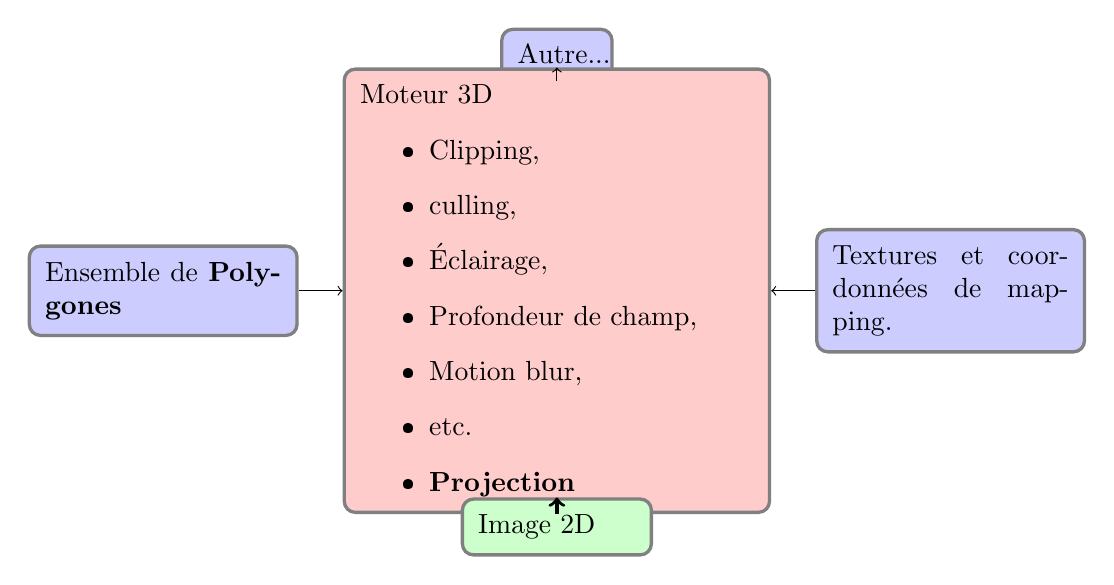
\begin{tikzpicture}
  [entree/.style={
    draw=black!50,
    fill=blue!20,
    rectangle,
    rounded corners,
    inner sep=.2cm,
    very thick}, systeme/.style={
    draw=black!50,
    fill=red!20,
    rectangle,
    rounded corners,
    inner sep=.2cm,
    very thick}, sortie/.style={
    draw=black!50,
    fill=green!20,
    rectangle,
    rounded corners,
    inner sep=.2cm,
    very thick}]

  \node [entree] at (-5,0) (polygone) {
  \begin{minipage}{3cm}
    Ensemble de \textbf{Polygones}
  \end{minipage}
  };

  \node [entree] at (5,0) (textures) {
  \begin{minipage}{3cm}
    Textures et coordonnées de mapping.
  \end{minipage}
  };

  \node [entree] at (0,3) (other) {
  \begin{minipage}{1cm}
    Autre...
  \end{minipage}
  };

  \node [systeme] (engine) {
  \begin{minipage}{5cm}
    Moteur 3D 
    \begin{itemize}
      \item Clipping,
      \item culling,
      \item Éclairage,
      \item Profondeur de champ,
      \item Motion blur,
      \item etc.
      \item \textbf{Projection}
    \end{itemize}
  \end{minipage}
  };

  \node [sortie] at (0,-3) (image) {
  \begin{minipage}{2cm}
    Image 2D
  \end{minipage}
  };

  \draw [->] (polygone) -- (engine);
  \draw [->] (textures) -- (engine);
  \draw [->] (other) -- (engine);
  \draw [very thick, ->] (engine) -- (image);
\end{tikzpicture}
\caption{Représentation grossière du pipeline de rendu via la
rasterisation\label{rasterisationPipeline}}
\end{center}

\end{figure}


L'avantage de cette technique vient du fait que les calculs sont très aisément
parallélisables. En effet, la même opération est répétée sur chaque sommet à
tracer. Nous assistons d'ailleurs à un développement de la technologie dans ce
sens : les \glspl{GPU} sont devenus de vraies collections de processeurs !\\

Hélas, cette technique n'offre pas que des avantages. En effet, la
complexification des scènes et surtout la demande du publique pour des rendus
encore plus réalistes poussent matériel et logiciel dans leur retranchement.
Les ingénieurs doivent désormais rivaliser d'ingéniosité en créer des
\glspl{shader} de plus en plus compliqués et gourmands.\\

Heureusement, depuis plus de 30 ans sous l'impulsion de \cite{Whitted1980},
chercheurs et ingénieurs développent une technique de rendu conceptuellement
simple mais très puissante : le \raytracing{}\ !
